%!TEX program = xelatex

\documentclass[compress]{beamer}
%--------------------------------------------------------------------------
% Common packages
%--------------------------------------------------------------------------

\definecolor{links}{HTML}{663000}
\hypersetup{colorlinks,linkcolor=,urlcolor=links}

\usepackage[english]{babel}
\usepackage{pgfpages} % required for notes on second screen
\usepackage{graphicx}

\usepackage{pdfpcnotes}

\usepackage{multicol}

\usepackage{tabularx,ragged2e}
\usepackage{booktabs}

\setlength{\emergencystretch}{3em}  % prevent overfull lines
\providecommand{\tightlist}{%
  \setlength{\itemsep}{0pt}\setlength{\parskip}{0pt}}


\usetheme{hri}

% Display the navigation bullet even without subsections
\usepackage{remreset}% tiny package containing just the \@removefromreset command
\makeatletter
\@removefromreset{subsection}{section}
\makeatother
\setcounter{subsection}{1}

\makeatletter
\let\beamer@writeslidentry@miniframeson=\beamer@writeslidentry
\def\beamer@writeslidentry@miniframesoff{%
  \expandafter\beamer@ifempty\expandafter{\beamer@framestartpage}{}% does not happen normally
  {%else
    % removed \addtocontents commands
    \clearpage\beamer@notesactions%
  }
}
\newcommand*{\miniframeson}{\let\beamer@writeslidentry=\beamer@writeslidentry@miniframeson}
\newcommand*{\miniframesoff}{\let\beamer@writeslidentry=\beamer@writeslidentry@miniframesoff}
\makeatother



\newcommand{\source}[2]{{\tiny\it Source: \href{#1}{#2}}}

\usepackage{tikz}
\usetikzlibrary{mindmap,backgrounds,positioning,calc,patterns}
\usepackage{pgfplots}
\pgfplotsset{compat=newest}
\usepackage{circuitikz}

\graphicspath{{figs/}}

\title{ROCO222 \newline Intro to Sensors and Actuators}
\subtitle{Electromagnetism \& DC motor -- Part 2}

\date{}
\author{Séverin Lemaignan}
\institute{Centre for Robotics and Neural Systems\\{\bf Plymouth University}}

\begin{document}


%%%%%%%%%%%%%%%%%%%%%%%%%%%%%%%%%%%%%%%%%%%%%%%%%%%%%%%%

\licenseframe{github.com/severin-lemaignan/module-introduction-sensors-actuators}

%%%%%%%%%%%%%%%%%%%%%%%%%%%%%%%%%%%%%%%%%%%%%%%%%%%%%%%%

\maketitle

\miniframesoff
\begin{frame}[fragile]{Last week's programming challenge}

Code a \sh{trumpsays} in Python:

\begin{verbatim}
$ trumpsays "Being nice to Rocket Man has failed."
   ,------._      ________________________
  /         :    /                        \
 /  ,-__-.  :   | Being nice to Rocket Man |
; ,' _   _`-|  /  has failed.              |
|/  - ||-   | / __________________________/
|\   /_\    |---
:|         |;
 \    O    ;
  \        ;
   `--+---'
\end{verbatim}

\end{frame}

\begin{frame}[fragile]{}
\begin{pythoncode}
#! /usr/bin/python

import sys
text = sys.argv[1] # retrieve the first command-line parameter

def go(line):
    """ move the console cursor to the start of a balloon's line.
    Uses ANSI escape codes: https://en.wikipedia.org/wiki/ANSI_escape_code
    """
    sys.stdout.write("\033[u\033[" + str(9-line) + "A\033[G\033[17C")

balloon_length = 24
trump = """
   ,------._     
  /         :    ________________________
 /  ,-__-.  :   /                        \\  
; ,' _   _`-|  /  
|/  - ||-   | /  
|\   /_\    |---
:|         |;
 \    O    ;
  \        ;
   `--+---'
"""
print(trump)
print("\033[s") # save the cursor position (bottom of the screen)
\end{pythoncode}
\end{frame}

\begin{frame}[fragile]{}
\begin{pythoncode}
go(0)

line = 0
current_length = 0 # holds the nb of characters printed on current line
for word in text.split(" "): # iterate over each of the words 

    # do we need a line break?
    if current_length + len(word) >= balloon_length:
        line += 1
        go(line)
        current_length = 0

    current_length += len(word) + 1
    sys.stdout.write(word + " ") # print the word, without final line break

# Draw the balloon contours
for i in range(line+1):
    go(i)
    sys.stdout.write("\033[2D|\033[" + str(balloon_length + 2) + "C|")

go(line + 1)
sys.stdout.write("\033[D\\" + "_" * balloon_length + "/")

print("\033[u") # restore the position of the cursor, to the bottom
\end{pythoncode}


\end{frame}

\begin{frame}[fragile]{This week's challenge}

    \Large
    Console-based image viewer

        \begin{center}
            
\includegraphics[width=0.7\linewidth]{coding-challenge-terminal-image}
        \end{center}

\end{frame}

\begin{frame}[fragile]{Tips for this week's challenge}
\begin{pythoncode}
# how to get the pixels of an image?
from PIL import Image
im = Image.open('image.jpg')
rgb_im = im.convert('RGB')
r, g, b = rgb_im.getpixel((1, 1))


# use ANSI escape code to set the adequate foreground/background color
# see https://en.wikipedia.org/wiki/ANSI_escape_code#24-bit

# use in a clever way the Unicode character U+2580, 'Upper Half Block'
# to increase the resolution of your viewer
\end{pythoncode}

\end{frame}

\miniframeson


%%%%%%%%%%%%%%%%%%%%%%%%%%%%%%%%%%%%%%%%%%%%%%%%%%%%%%%%


\miniframesoff

\section[]{So far in electromagnetism...}

\begin{frame}{Recap of last lecture}
    \begin{itemize}
        \item Ampère's law: $\displaystyle\oint \vec{B} \cdot d\vec{l} = \mu_0 \cdot I$
        \item Faraday's law of induction: $\displaystyle\mathcal{E} = -N \cdot
            \frac{d\Phi_B}{dt}$ (with $\Phi_B = B\cdot A \cdot cos(\theta)$ iff
            $\vec{B}$ is uniform)
        \item Lenz law: (the minus in Faraday's law)
        \item Lorentz law: $\displaystyle \vec{F} = \vec{I} \cdot L \times \vec{B}$
    \end{itemize}
\end{frame}

\begin{frame}{Today's objectives}

    \begin{itemize}
        \item Understand and know how to characterise \textbf{electrical inductance}
        \item Describe a motor from \textbf{its equivalent circuit}
        \item \textbf{Relate a motor's angular velocity to voltage and torque}
        \item Model the motor's \textbf{dynamics} and use \textbf{Laplace
            transforms} to solve the motor differential equations
        \item Know how to read and interpret a \textbf{motor datasheet}
        \item Undertand the working principle of a \textbf{brushless motor} and
            how it compares to brushed DC motors
    \end{itemize}
\end{frame}
\miniframeson



\section{Inductance}

{\fullbackground[scale=0.9,page=39]{ian-electromagnetism.pdf}
    \begin{frame}{Electrical resistance}
    \end{frame}
}

{\fullbackground[scale=0.9,page=40]{ian-electromagnetism.pdf}
    \begin{frame}{Electrical inductance}
    \end{frame}
}

\begin{frame}{Current in an LR circuit}
    \begin{columns}
        \begin{column}{0.5\linewidth}
            \begin{align*}
                V &= V_R + V_L \\
                V_R &= I \cdot R \\
                V_L &= L \cdot \frac{dI}{dt} \\
                \Rightarrow V &= I \cdot R + L \cdot \frac{dI}{dt} \\
            \end{align*}
        \end{column}
        \begin{column}{0.5\linewidth}
        \begin{center}
            \resizebox{\linewidth}{!}{
                \begin{circuitikz}
                    \draw
                    (0,0) to [open, v^>=$V$] (0,3) 
                    to [short, *- ,i=$I$] (1,3) 
                    to [R, l=$R$] (3,3) 
                    to [L, l=$L$] (3,0)
                    to [short, -*] (0,0);
                \end{circuitikz}
            }
        \end{center}
        \end{column}
    \end{columns}

    \begin{center}
        This is a first-order linear differential equation.
    \end{center}
\end{frame}

{\fullbackground[scale=0.9,page=42]{ian-electromagnetism.pdf}
    \begin{frame}{Current in an LR circuit}
    \end{frame}
}

{\fullbackground[scale=0.9,page=43]{ian-electromagnetism.pdf}
    \begin{frame}{Definition of inductance}
    \end{frame}
}

{\fullbackground[scale=0.9,page=44]{ian-electromagnetism.pdf}
    \begin{frame}{Inductance of a solenoid}
    \end{frame}
}


\begin{frame}{Consequence for motors}

    \only<1>{
  Moving a magnet in a coil induces current:


    \begin{center}
        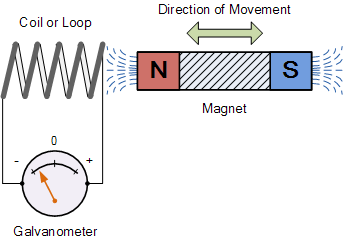
\includegraphics[width=0.6\linewidth]{image29}

    \scalebox{1.5}{Faraday's law of induction: $\displaystyle\mathcal{E} = - \frac{d\Phi_B}{dt}$}

    \end{center}
}

    \only<2>{
        
    If a coil consists of N loops with the same area, the total induced EMF in
    the coil is given by:

\[
        \mathcal{E} = -N \cdot \frac{d\Phi_B}{dt}
\]

In a uniform magnetic field, the induced EMF can be expressed as:

\[
    \mathcal{E} = -N \cdot \frac{d}{dt} (B A cos(\theta)) = - N \cdot B \cdot A \frac{d cos(\theta)}{dt} = -N \cdot B \cdot A \cdot sin(\theta) \cdot \dot\theta
\]

With enough coils,

\[
    \mathcal{E} = - N \cdot B \cdot A \cdot \dot\theta = - K_e \dot\theta
\]

    $K_e$ is the \textbf{back-EMF} constant of the motor.


    }
\end{frame}

%%%%%%%%%%%%%%%%%%%%%%%%%%%%%%%%%%%%%%%%%%%%%%%%%%%%%%%%%%%%%%%%%%%%%%%%%%%%%%%%%%%%%%%%%%%%%%%%
%%%%%%%%%%%%%%%%%%%%%%%%%%%%%%%%%%%%%%%%%%%%%%%%%%%%%%%%%%%%%%%%%%%%%%%%%%%%%%%%%%%%%%%%%%%%%%%%
\section[Voltage]{Voltage in a motor}

\begin{frame}{Electrical generator}

    \begin{center}
        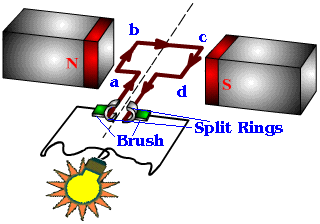
\includegraphics[width=0.6\linewidth]{image30}
    \end{center}

\begin{itemize}

\item Speed of rotation affects voltage generated
\item So how fast will a motor rotate with applied voltage $V$?
\item Lets consider the equivalent circuit for a DC motor
\end{itemize}
\end{frame}

\begin{frame}{DC motor equivalent circuit}

    \begin{center}
        \resizebox{0.6\linewidth}{!}{
            % Based on http://texample.net/tikz/examples/induction-machine/
            \begin{circuitikz}
                \draw
                % rotor circuit
                (0,0) to [short, *-] (6,0)
                to [V, l_={EMF}] (6,2) % rotor emf

                % stator circuit
                (0,0) to [open, v^>=$V$] (0,2) % stator voltage
                to [short, *- ,i=$I$] (1,2) % stator current
                to [R, l=$R$] (3,2) % stator resistance
                to [L, l=$L$] (6,2); % leakage inductance
            \end{circuitikz}
        }
    \end{center}

\footnotesize
\begin{itemize}

\item $V$ is the applied voltage, $I$ is the drawn current
\item Resistance $R$ arises from the coil and the brushes
\item Inductance $L$ arises from the coil
\item Back EMF arises from rotation of the coil in the magnetic field
  created by the stator magnets
\end{itemize}

\end{frame}

\begin{frame}{Voltage in a DC motor}

    \begin{center}
        \resizebox{0.6\linewidth}{!}{
            % Based on http://texample.net/tikz/examples/induction-machine/
            \begin{circuitikz}
                \draw
                % rotor circuit
                (0,0) to [short, *-] (6,0)
                to [V, l_={EMF $\mathcal{E}$}] (6,2) % rotor emf

                % stator circuit
                (0,0) to [open, v^>=$V$] (0,2) % stator voltage
                to [short, *- ,i=$I$] (1,2) % stator current
                to [R, l=$R$] (3,2) % stator resistance
                to [L, l=$L$] (6,2); % leakage inductance
            \end{circuitikz}
        }
    \end{center}

\textbf{Kirchhoff's voltage law}: voltage across resistor, inductance and
back EMF balance applied voltage

\begin{align*}
    V &= I \cdot R + L \cdot \frac{dI}{dt} + \mathcal{E} \\
      &= I \cdot R + L \cdot \frac{dI}{dt} - K_e \cdot \dot\theta
\end{align*}

\pause

How to know $I$?

\end{frame}


\begin{frame}{Conservation of energy!}


    \textbf{Conservation of energy means electrical power in = mechanical power out +
    losses}



    \begin{columns}
        \begin{column}{0.7\linewidth}
    \begin{center}
        \resizebox{0.9\linewidth}{!}{
            \begin{tikzpicture}[>=latex]

                \node at (0,0) (motor) {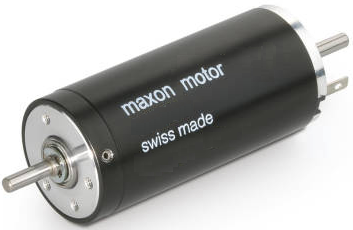
\includegraphics[width=3cm]{../part2/figs/maxon}};
                \node[below left=0.5 of motor] (pmech) {$P_{mech}= \tau \cdot \dot\theta$};
                \node[above right=0.5 of motor] (pel) {$P_{el}= V \cdot I$};
                \node[below right=0.5 of motor] (pr) {$P_{r}=R \cdot I^2$};
                \draw[ultra thick, red,->] (motor) -- (pmech);
                \draw[ultra thick, red,->] (pel) -- (motor);
                \draw[ultra thick, orange,->] (motor) -- (pr);
            \end{tikzpicture}
        }

    \end{center}

        \end{column}
        \begin{column}{0.3\linewidth}
    \footnotesize
    where:

        $\tau$ = torque;
        
        $\dot\theta$ = angular velocity;
        
        $I$ = input current;
        
        $V$ = applied voltage;

        $R$ = windings resistance
            
        \end{column}
    \end{columns}

        \begin{center}
    \[
        P_{el} = P_{mech} + P_{r}
    \]
        \end{center}

\end{frame}


\begin{frame}{Remember torque}

\only<1>{
    \begin{center}
        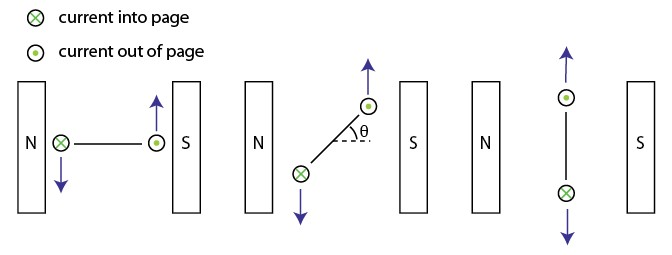
\includegraphics[width=0.8\linewidth]{../part2/figs/image16-3}
    \end{center}

If current $I$ flows through a coil of depth $L$ and width $d$ with $N$ turns,
    with magnetic field $B$, the coil pivots and generates a torque $\tau$ given
    by:

\[
\tau = N \cdot 2 (\frac{d}{2}) \cdot F \cdot cos(\theta) = N \cdot d \cdot B \cdot I \cdot L \cdot cos(\theta)
\]
}

    \only<2>{
With enough coils, we can remove the $cos(\theta)$ term:
\[
\tau = N \cdot d \cdot B \cdot I \cdot L = K_\tau \cdot I
\]


$K_\tau$ is the motor's torque constant.

}

\end{frame}

\begin{frame}{Putting it all together}

    \begin{columns}
        \begin{column}{0.5\linewidth}

    \begin{itemize}
        \item $V = - K_e \cdot \dot\theta + I \cdot R$
        \item $\tau = K_\tau \cdot I$

    \end{itemize}
        \end{column}
        \begin{column}{0.5\linewidth}
    $V$ = applied voltage
            
    $\dot\theta$ = motor angular velocity
            
    $I$ = motor current
    
    $R$ = motor resistance
    
    $\tau$ = torque, including frictional losses
        \end{column}
    \end{columns}


    \pause 

    \begin{itemize}
        \item Electrical power in: $V \cdot I = - K_e \cdot \dot\theta \cdot I + I^2 \cdot R$
        \item Mechanical power out: $\tau \cdot \dot\theta = K_\tau \cdot I \cdot \dot\theta$
        \item Losses: $I^2 \cdot R$
    \end{itemize}

    \pause

    Conservation of energy means electrical power in = mechanical power out +
    losses.

    This is true if and only if $K_e=K_\tau$.

    \pause

    \textbf{In a DC motor, the torque constant and back-EMF constants are equal.}
\end{frame}

\begin{frame}{Back to the voltage}


\begin{align*}
    V &= K_e \cdot \dot\theta + I \cdot R \\
    \tau &= K_\tau \cdot I \Rightarrow I = \frac{\tau}{K_\tau}
\end{align*}

\Large
\begin{equation*}
\begin{split}
    \Rightarrow V &= \frac{\tau}{K_\tau} \cdot R + K_e \cdot \dot\theta \\
    \Rightarrow \dot\theta &= \frac{V\bubblemark{voltage}}{K} - R \cdot \frac{\tau\bubblemark{torque}}{K^2}
\end{split}
\end{equation*}

\bubble<2>[-10][2][2cm]{voltage}{Speed is a linear function of both voltage...}
\bubble<2>[190][2][2cm]{torque}{...and torque}
\end{frame}


\begin{frame}{Motor constants}

\begin{align*}
    \mathcal{E} &= - N \cdot B \cdot A \cdot \dot\theta = - K_e \cdot \dot\theta \\
    \Rightarrow K_e &= N \cdot B \cdot A
\end{align*}

\begin{align*}
    \tau &= N \cdot d \cdot B \cdot I \cdot L = K_\tau \cdot I \\
    \Rightarrow K_\tau &= N\bubblemark{turns} \cdot d\bubblemark{width} \cdot B\bubblemark{magneticfield} \cdot L\bubblemark{length}
\end{align*}

\bubble<1->[10][3][2cm]{turns}{turns per coil}
\bubble<1->[50][1][2cm]{width}{coil width}
\bubble<1->[130][1][2cm]{magneticfield}{permanent magnetic field}
\bubble<1->[170][3][2cm]{length}{coil length}

\pause

\begin{align*}
    K_e &= K_\tau \\
    \Rightarrow N \cdot B \cdot A &= N \cdot d \cdot B \cdot L
\end{align*}

\end{frame}

\begin{frame}{How to choose the motor constants?}

\begin{align*}
    V &= I \cdot R + L \cdot \frac{dI}{dt} - K_e \cdot \dot\theta \\
    \mathcal{E} &= - K_e \cdot \dot\theta \\
    \tau &= K_\tau \cdot I \\
\end{align*}

    \only<1>{
    If you pick a $K_\tau=K_e$ \textbf{too high}, you `run out of voltage' and
    \textbf{can not achieve the speed you need}. 

    If you pick a $K_\tau=K_e$ \textbf{too low}, the current needed to achieve
    the torque you need will be higher than necessary.
}
    \only<2>{
    Rule of thumb with DC motor selection: \textbf{pick a motor with a $K_\tau$ and
    back-EMF constant $K_e$ such that the supply voltage you have available is
    well-matched with the back-EMF at your maximum speed}.
}

    \source{https://electronics.stackexchange.com/questions/33315/understanding-motor-constants-kt-and-kemf-for-comparing-brushless-dc-motors}{stackexchange}
\end{frame}

%%%%%%%%%%%%%%%%%%%%%%%%%%%%%%%%%%%%%%%%%%%%%%%%%%%%%%%%%%%%%%%%%%%%%%%%%%%%%%%%%%%%%%%5
%%%%%%%%%%%%%%%%%%%%%%%%%%%%%%%%%%%%%%%%%%%%%%%%%%%%%%%%%%%%%%%%%%%%%%%%%%%%%%%%%%%%%%%5
%%%%%%%%%%%%%%%%%%%%%%%%%%%%%%%%%%%%%%%%%%%%%%%%%%%%%%%%%%%%%%%%%%%%%%%%%%%%%%%%%%%%%%%5

\section[Motor dynamics]{DC motor dynamics}


\begin{frame}{DC motor dynamics}

    \Large
    So far, we have been considering the motor in \textbf{steady state}: the
    current, the voltage, the angular velocity do not change over time.

    \hspace{2em}

    What about the dynamics?

    \only<1>{

        \begin{center}
            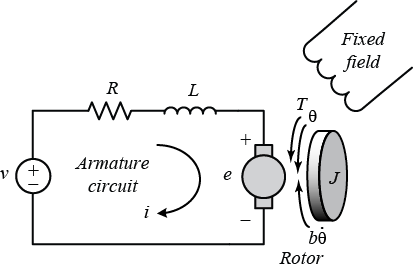
\includegraphics[width=0.5\linewidth]{image63}
        \end{center}

    }

    \only<2>{
        Notation:

        \begin{itemize}
            \item $I \rightarrow i(t)$
            \item $V \rightarrow v(t)$
            \item $\theta \rightarrow \theta(t)$
        \end{itemize}
    }
\end{frame}

\begin{frame}{Moment of Inertia}

    Resists with opposing torque proportional to angular acceleration

    \begin{columns}
        \begin{column}{0.5\linewidth}
            \begin{center}
                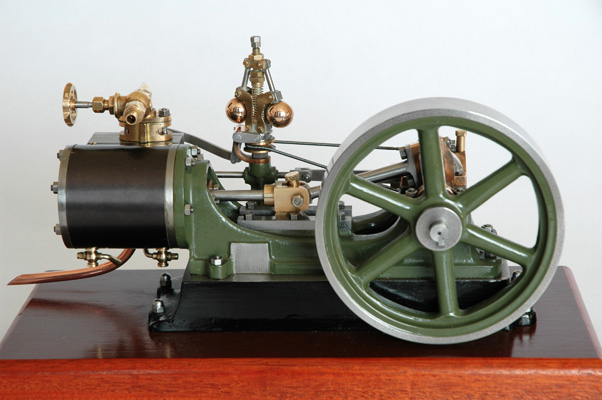
\includegraphics[height=0.4\paperheight]{image62}
            \end{center}

            where

            $\tau$ is the torque, in $N\cdot m$

            $J$ is the moment of inertia, in $kg \cdot m^2$

        \end{column}
        \begin{column}{0.5\linewidth}
            \begin{center}
                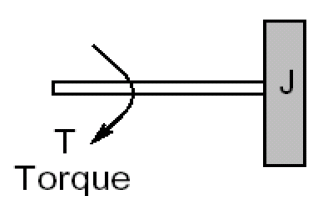
\includegraphics[width=0.8\linewidth]{torque}

            \Huge
            $\displaystyle\tau = J \cdot \frac{d^2 \theta}{dt^2}$
            \end{center}
        \end{column}
    \end{columns}

\end{frame}

\begin{frame}{DC motor dynamics}

    \begin{center}
        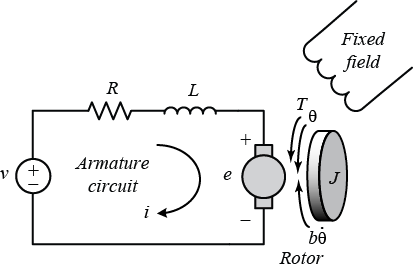
\includegraphics[width=0.5\linewidth]{image63}
    \end{center}

\only<1> {
\begin{itemize}

\item $R$ = Armature resistance (in ohms $\Omega$)
\item $L$ = Armature inductance (in Henrys $H$) % CHECK
\item $J$ = Moment of inertia for the motor rotor ($kg\cdot m^2$)
\item $b$ = Motor viscous friction constant (in $N\cdot m\cdot s$)
\item $K_t$ = Motor torque constant (in $\frac{N\cdot m}{A}$)
\item $K_e$ = Electromotive force constant (in $\frac{V\cdot rad^{-1}}{sec}$) % CHECK
\end{itemize}
}

    \only<2> {
    Motor torque $\tau_m$ is given by $\tau_m = K_\tau \cdot i(t)$

Mechanical resisting torque $\tau_r$ is given by $\tau_r = b \cdot \dot\theta + J \cdot \ddot\theta$

Under no load, $\tau_m = \tau_r$

Therefore:
\[
    K_\tau \cdot i(t) = b \cdot \dot\theta + J \cdot \ddot\theta
\]

}
    \only<3> {

\textbf{Kirchhoff's voltage law}: voltage across resistor, inductance and
back EMF balance applied voltage

    \[
        v(t) = i(t) \cdot R + L \cdot \frac{di}{dt} - K_e \cdot \dot\theta
    \]
}
\end{frame}

\begin{frame}{Differential equation of a DC motor}

    \Large
\begin{align*}
    \only<1->{
        K \cdot i(t) &= b \cdot \dot\theta + J \cdot \ddot\theta \\
            v(t) &= i(t) \cdot R + L \cdot \frac{di}{dt} - K \cdot \dot\theta \\
    }
    \only<2->{
    \Rightarrow v(t) &= (\frac{b}{K} - K) \cdot \dot\theta + \frac{J}{K} \cdot \ddot\theta + L \frac{d (\frac{b}{K} \cdot \dot\theta + \frac{J}{K} \cdot \ddot\theta)}{dt} \\
    }
    \only<3->{
        \Rightarrow v(t) &= (\frac{b}{K} - K) \cdot \dot\theta + (\frac{J}{K} + \frac{L\cdot b}{K}) \cdot \ddot\theta + \frac{L \cdot J}{K} \cdot \dddot\theta
}
\end{align*}

    \only<3-> {
\normalsize
We can integrate 3 times, or...
}

\end{frame}

\begin{frame}{Laplace transform}

    \only<1>{
The Laplace transform is a linear operator that maps a function $f(t)$ to
$F(s)$ in the frequency domain.


Specifically:

\[
    F(s) = \mathcal{L}\{f\}(s) =  \mathcal{L}\{f(t)\} = \int^{\inf}_{0} f(t)e^{-st}dt
\]

where $s = \sigma + i\omega$ (the complex number frequency parameter)

    Go from a function of a \emph{real} variable (here time $t$) to a complex
    function of a complex variable (frequency, $s$).

}

    \only<2> {

        Why bother?

        Often \textbf{simplifies the process of analyzing the behavior of the
        system}.

        For example, Laplace transformation from the time domain to the
        frequency domain \textbf{transforms differential equations into algebraic
        equations}.
    }
\end{frame}

\begin{frame}{Operations useful for solving differential equations}

\Large

\[
    \mathcal{L} \{f'(t)\} = sF(s) - f(0)
\]


\[
    \mathcal{L} \{f''(t)\} = s^2F(s) - sf(0) - f'(0)
\]


\[
    \mathcal{L} \{\int^{t}_{0}f(t)dt\} = \frac{F(s)}{s}
\]

\vspace{2em}
\small
See
    \href{https://en.wikipedia.org/wiki/Laplace_transform}{Wikipedia}
    for more properties.

\end{frame}

\begin{frame}{Solution using Laplace transformations}

\only<1>{

Taking Laplace transforms of the differential equations that describe
the motor mechanical dynamics:

\[
   K \cdot i(t) = b \cdot \dot\theta + J \cdot \ddot\theta
\]

becomes:

\[
    K \cdot I(s) = b \cdot s \cdot \theta(s) + J \cdot s^2 \cdot \theta(s)
\]

\[
    I(s) = \frac{s \cdot (b + J \cdot s) \cdot \theta(s)}{K}
\]

}

    \only<2> {

Taking Laplace transforms of the differential equations that describe
the motor voltages:

\[
        v(t) = i(t) \cdot R + L \cdot \frac{di}{dt} + K \cdot \dot\theta
\]

becomes:

\[
    V(s) = I(s) \cdot (R + L\cdot s) + K \cdot s \cdot \theta(s)
\]
}

    \only<3>{

Substituting:

\[
    I(s) = \frac{s \cdot (b + J \cdot s) \cdot \theta(s)}{K}
\]


into:

\[
    V(s) = I(s) \cdot (R + L\cdot s) + K \cdot s \cdot \theta(s)
\]

by eliminating current $I(s)$ gives:

\[
    \theta(s) = \frac{K}{s \cdot ( (J \cdot s + b) \cdot (L \cdot s+ R) + K^2)} \cdot V(s)
\]

}

\end{frame}

\begin{frame}{Transfer function}

    \begin{columns}
        \begin{column}{0.5\linewidth}

            Result of a transfer response output position for a DC electric motor
            given its input voltage

        \end{column}
        \begin{column}{0.5\linewidth}


            \begin{center}
                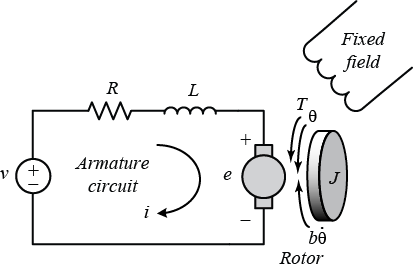
\includegraphics[width=0.9\columnwidth]{image63}
            \end{center}

        \end{column}
    \end{columns}

\[
    \theta(s) = \frac{K}{s \cdot ( (J \cdot s + b) \cdot (L \cdot s+ R) + K^2)} \cdot V(s)
\]

\pause

We can differentiate this expression to get the transfer function for speed

\[
    \dot\theta(s) = \frac{K}{(J \cdot s + b) \cdot (L \cdot s + R) + K^2} \cdot V(s)
\]


\end{frame}

%%%%%%%%%%%%%%%%%%%%%%%%%%%%%%%%%%%%%%%%%%%%%%%%%%%%%%%%%%%%%%%%%%%%%%%%%%%%%%%%%%%%%%%%%%%%%%%%%%%%
%%%%%%%%%%%%%%%%%%%%%%%%%%%%%%%%%%%%%%%%%%%%%%%%%%%%%%%%%%%%%%%%%%%%%%%%%%%%%%%%%%%%%%%%%%%%%%%%%%%%
%%%%%%%%%%%%%%%%%%%%%%%%%%%%%%%%%%%%%%%%%%%%%%%%%%%%%%%%%%%%%%%%%%%%%%%%%%%%%%%%%%%%%%%%%%%%%%%%%%%%
\miniframesoff
\begin{frame}[plain]
    \begin{center}
        \Large
        10 min break\\[2em]
    \end{center}
\end{frame}
\miniframeson

%%%%%%%%%%%%%%%%%%%%%%%%%%%%%%%%%%%%%%%%%%%%%%%%%%%%%%%%%%%%%%%%%%%%%%%%%%%%%%%%%%%%%%%%%%%%%%%%%%%%
%%%%%%%%%%%%%%%%%%%%%%%%%%%%%%%%%%%%%%%%%%%%%%%%%%%%%%%%%%%%%%%%%%%%%%%%%%%%%%%%%%%%%%%%%%%%%%%%%%%%
%%%%%%%%%%%%%%%%%%%%%%%%%%%%%%%%%%%%%%%%%%%%%%%%%%%%%%%%%%%%%%%%%%%%%%%%%%%%%%%%%%%%%%%%%%%%%%%%%%%%

\section[Datasheets]{Wrap-up on DC motors: another look at datasheets}

{\fullbackground[scale=0.9,page=2]{ian-dc-motor-datasheet.pdf}
    \begin{frame}{Maxon DC motor variants}

        \pnote{
            What are the differences of the different maxon motors?

        Basic possibilities for variation
        different magnetic materials: AlNiCo, NdFeB, ferrite, …
        Commutation: Graphite brushes or precious metal brushes
        Bearings: Sintered sleeve bearings or ball bearings

        The motor family reflects the magnet type used: e.g. RE motors have NdFeB
        magnets.
        Depending on operation conditions and power each DC motor type can be
        equipped with either bearing or commutation type.

        }
    \end{frame}
}

\begin{frame}{Development of permanent magnets}
    \begin{center}
        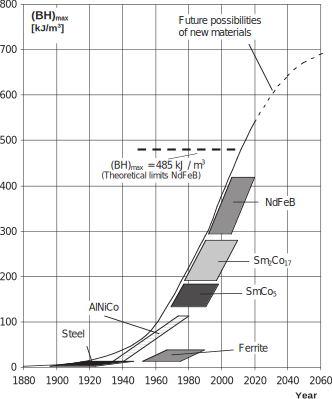
\includegraphics[height=0.7\paperheight]{permanent-magnets}

        \source{http://www.vacuumschmelze.com/fileadmin/Medienbiliothek_2010/Downloads/DM/VACODYM-VACOMAX-PD002_2015_en.pdf}{vacuumschmelze}
    \end{center}

    \pnote{
        A few words about permanent magnets.
        This slides shoes the development of the power density of permanent
        magnets in the last century
        It all started with magnetic steels from which the AlNiCo magnets
        evolved in the middle of the century becoming the strongest magnet
        material. Improved manufacturing processes in the 60ies allowed to
        create an internal structure, an anisotropic axis. This further enhanced
        the energy product. This material together with the ferrites was at the
        base of the development of small permanent magnet DC motors. The higher
        energy density of AlNiCo compared to the ferrites was reflected in the
        higher power density of coreless DC motors compared to conventional DC
        motors
        In the 70ies the first rare earth magnets based on Samarium and cobalt
        appeared. They wer much stronger than AlNiCo. In the 80ies the even
        stronger Neodymium-Iron-Boron magnets emerged on the market. Only
        ironless designs can make the full use of their strength resulting in
        the extremelx high power density of coreless DC motors.

        However, power density is just one parameter among others in magnetic
        applications.
        The magnets should be able to be easily magnetized
        In motors the magnets must support the heat without loosing power or
        change irreversibly.
        Mechanical stability, ease of manufacturing, corrosion resistance are
        further important features.
        And of course the cost. In DC motors the magnet cost can amount to as
        much as 40\%.

        Newer, stronger materials that can be produced and machined reasonably
        don't seem to appear in the next future. The developments point rather
        in the direction of improving thermal and chemical stability and
        enhancing the remanence of existing magnets.
    }
\end{frame}

%{\fullbackground[scale=0.9,page=4]{ian-dc-motor-datasheet.pdf}
%    \begin{frame}{Permanent magnets}
%
%        \pnote{
%        This diagram shows the areas where the typical demagnetization curves of
%        different magnetic materials lie.
%
%        On the vertical axis we have the magnetization (or more precisely the
%        magnetic flux density B), to the left we have the external demagnetization
%        field H, pointing in the opposite direction. Magnetization decreases
%        with increasing field H.
%
%        The magnetization at zero external field is called remanence or residual
%        magnetism. It tells you how much a magnet can be magnetized. One can see
%        that AlNiCo and NdFeB can have a very high remanence of more than 1.2
%        Tesla.
%
%        The field H where the magnetization or magnetic induction vanishes is
%        called coercive field. One can see that rare earth magnets have a very
%        high coercive field which means they are difficult to demagnetize.
%
%        Increasing the air gap in a motor has a similar effect as increasing the
%        demagnetization field. In AlNiCo motors with the very steep
%        demagnetization curve only narrow air gaps can be made in order to have
%        a considerable magnetic induction. Accordingly the coreless winding has
%        a very thin wall thickness.
%
%        In RE motors the air gap can be made much larger. The winding is thicker
%        and the motor as a whole is stronger. (These effects quite nicely show
%        what's behind the "energy product" of permanent magnets.)
%        }
%
%    \end{frame}
%}

{\fullbackground[scale=0.9,page=5]{ian-dc-motor-datasheet.pdf}
    \begin{frame}{Understanding motor datasheets}
    \end{frame}
}

{\fullbackground[scale=0.9,page=6]{ian-dc-motor-datasheet.pdf}
    \begin{frame}{DC motor data}
    \end{frame}
}

\begin{frame}{Speed-torque characteristic}

    \begin{columns}
        \begin{column}{0.7\linewidth}
    \begin{center}
        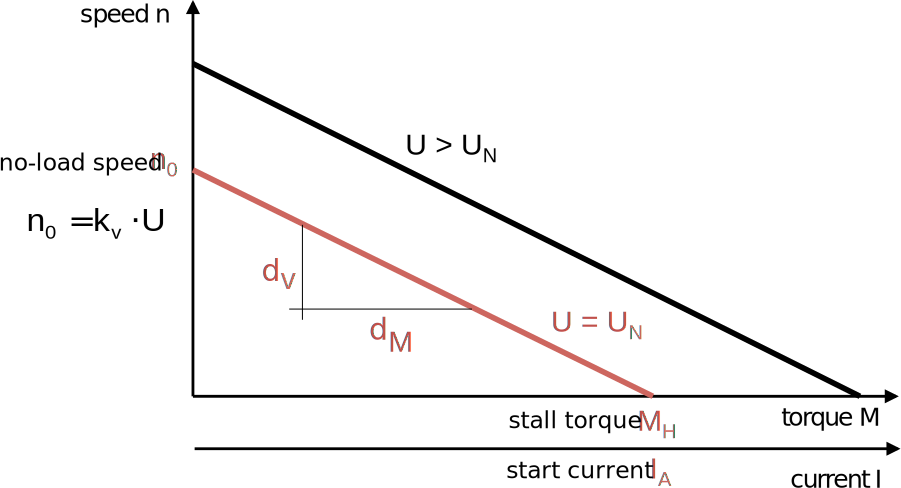
\includegraphics[width=\linewidth]{voltage-torque}
    \end{center}


        \end{column}
        \begin{column}{0.3\linewidth}
            Remember:

    \begin{align*}
        \dot\theta &= \frac{V}{K} - R \cdot \frac{\tau}{K^2} \\
        \tau &= K \cdot I
    \end{align*}

        \end{column}
    \end{columns}

    \pause
    Influence of voltage:

    \begin{itemize}
            \small
        \item no-load speed $n_0$ proportional to applied voltage
        \item stall torque $M_H$ proportional to the applied voltage
        \item increasing voltage shifts the speed-torque line upwards
        \item speed-torque gradient $\frac{d_v}{d_M}$ unaffected
    \end{itemize}

    \pnote{
    The relationship between speed and torque is the equation of a straight line in
    our standard representation where the speed is traced as a function of the
    torque (red line).

    At zero torque, the speed is highest. This speed is called no-load speed
    n0. The no-load speed can easily be calculated from the applied voltage
    and the speed constant of the motor.

    Enhancing the load torque leads to a linear reduction of the speed. It
    becomes clear what the meaning of Dn/DM is: It's the gradient of the
    speed-torque line.
    Increasing the torque further reduces speed up to the point where the
    motor stops. The corresponding torque is called stall torque MH.
    We have learned that torque and current are equivalent. Hence, we can
    draw a current axis in parallel to the torque axis. The current
    corresponding to the stall torque is named starting current IA. 

    A different view on the speed-torque line is to look at the start-up of
    the motor, i.e. we start at the right end of the speed-torque line.
    Applying a voltage at zero speed results in a high current, the starting
    current; there is no back-EMF to counteract the applied voltage. The
    current produces a high torque that accelerates the motor, the induced
    voltage increases and less current can flow. Hence, the faster the motor
    turns, the less torque is produced. 

    All these considerations are valid for a fixed applied voltage U. What
    happens if the voltage is changed, e.g. at a higher voltage? The applied
    voltage has only an influence on the first term, which is the no-load
    speed. A higher voltage results in a higher no-load speed. The
    speed-torque gradient is unaffected. As a net result: Changing the
    applied voltage results in a parallel shift of the speed-torque line.

    Remark: An important feature of the speed-torque line is the fact that
    the produced torque is highest at start, which makes these motors very
    dynamic.
    }
\end{frame}

{\fullbackground[scale=0.9,page=8]{ian-dc-motor-datasheet.pdf}
    \begin{frame}{Speed-torque characteristic}
    \end{frame}
}

{\fullbackground[scale=0.9,page=9]{ian-dc-motor-datasheet.pdf}
    \begin{frame}{Operating points 1/2}
        \pnote{
        The values at nominal voltage basically reflect three special operating points
        on the speed-torque line at nominal voltage.
        The first point is the no-load operating point.
        The no-load speed is the resulting speed if no external output torque
        has to be delivered.
        The no-load current is the current needed to overcome internal losses,
        e.g. friction. (More on the next slide)

        The second operating point is the rated or nominal operating point. It
        is defined by the maximum permissible continuous current or nominal
        current. This is the maximum current at which the motor can be operated
        for long periods of time without overheating. 
        The rated or nominal torque is the motor torque corresponding to the
        nominal current.
        The nominal speed has no deeper meaning. It's just the resulting speed
        at this load.

        The last operating point on the far right is at stall or start.
        The stall torque describes at which load torque the motor stalls, when
        supplied with the nominal voltage.
        The starting current is the corresponding current, that will also be
        present just after powering the motor with the nominal voltage.
        }
    \end{frame}
}

\begin{frame}{Operating points 2/2}

    \begin{itemize}
        \item \textbf{Load operating points} are defined by the
            applications. They are characterised by a load speed $n_L$ at a
            given load torque $M_L$
        \item \textbf{Motor operating points} lie on the speed-torque line: select
            the voltage accordingly.
    \end{itemize}

    \begin{center}
        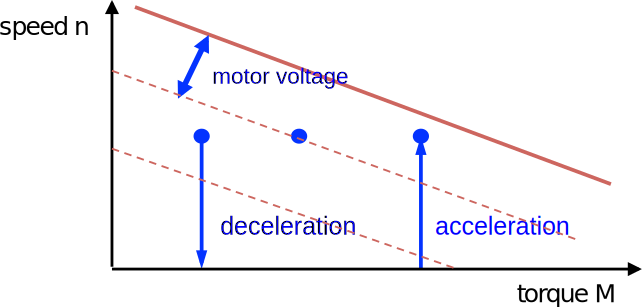
\includegraphics[width=0.8\linewidth]{operating-points}
    \end{center}

    \pnote{
    An important concept are the operating points. We have to distinguish between
    the Load operating points: These are pairs of speed and torque values that
    are required by application. In the diagram they are represented by the
    blue points. 
    Typically, during acceleration the highest torque is needed and all the
    points on the acceleration arrow are operating points that are run
    through. 
    The single point in the middle represents a constant motor operation at
    given load and speed.
    During deceleration, usually less torque is needed. Friction helps.
    The motor operating points are located on the speed-torque line at the
    relative voltage.

    Running the motor at the operating points demanded by the load requires
    the motor voltage to be adjusted correspondingly, and hence the
    speed-torque line. That's the task of a controller.
    }
\end{frame}

\begin{frame}{Effect of changing the windings}
    \[
    \dot\theta = \frac{V}{K} - R \cdot \frac{\tau}{K^2}
    \]

    \vspace{2em}
    ...what would be the effect?

    \begin{itemize}
        \item on max speed?
        \item on start current/stall torque?
    \end{itemize}

\end{frame}

{\fullbackground[scale=0.9,page=11]{ian-dc-motor-datasheet.pdf}
    \begin{frame}{Effect of changing the windings}
        \[
        \dot\theta = \frac{V}{K} - R \cdot \frac{\tau}{K^2}
        \]
    \vspace{\paperheight}
    \end{frame}
}

%{\fullbackground[scale=0.9,page=12]{ian-dc-motor-datasheet.pdf}
%    \begin{frame}{Torque constant $K_M$}
%    \end{frame}
%}
%
%{\fullbackground[scale=0.9,page=13]{ian-dc-motor-datasheet.pdf}
%    \begin{frame}{Torque constant $K_M$}
%    \end{frame}
%}
%
%{\fullbackground[scale=0.9,page=14]{ian-dc-motor-datasheet.pdf}
%    \begin{frame}{Speed constant $K_n$}
%    \end{frame}
%}

{\fullbackground[scale=0.9,page=15]{ian-dc-motor-datasheet.pdf}
    \begin{frame}{Nominal motor characteristics}
    \end{frame}
}

{\fullbackground[scale=0.9,page=16]{ian-dc-motor-datasheet.pdf}
    \begin{frame}{List of main motor parameters}
    \end{frame}
}

{\fullbackground[scale=0.9,page=17]{ian-dc-motor-datasheet.pdf}
    \begin{frame}{Motor thermal considerations}
    \end{frame}
}

{\fullbackground[scale=0.9,page=18]{ian-dc-motor-datasheet.pdf}
    \begin{frame}{Influence of temperature on motor operation}
        \pnote{
        Temperature has an influence on motor data as well. 

        Generally, the permanent magnets become weaker at higher temperature, but this
        is a reversible effect within the permissible temperature range of the
        motors; the magnets regain their original strength when they cool down. 
        AlNiCo magnets show the weakest temperature dependency. That's why they
        are used in DC Tachos, a measuring device that should give the same
        output independent of temperature.

        Neodymium magnets have a stronger temperature dependency. A motor that
        is 50°C hotter exhibits a speed constant that is about 5\% higher and a
        torque constant that is about 5\% lower.

        When the motor heats up, the winding resistance increases by about 0.4%
        per Kelvin. The main effect is that power losses will be even more
        pronounced at higher temperature.

        The variation of the motor data with temperature create problems in
        applications very seldom. Although motor selection is done with the data
        specified for the cold motor at room temperature, there is usually
        enough margin left to compensate for the weakening of the motor when it
        becomes hot in prolonged operation.
        }
    \end{frame}
}

\begin{frame}{Permissible torque and temperature}
    \begin{center}
        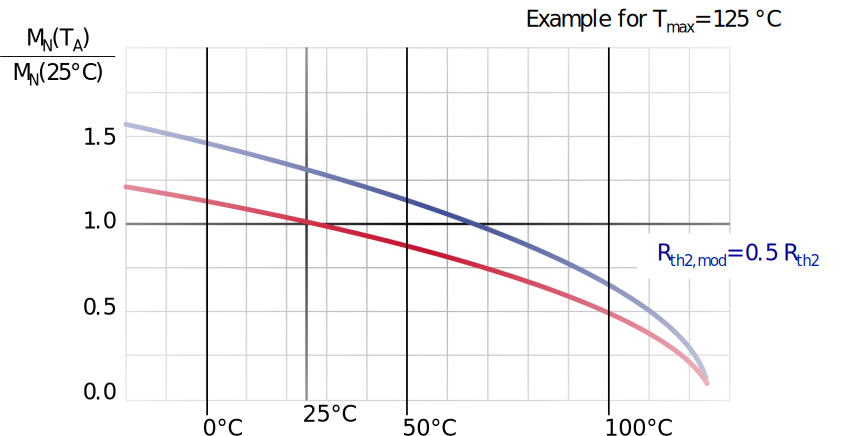
\includegraphics[width=\linewidth]{temperature-torque}
    \end{center}
    \pnote{
    This diagram shows the influence of the ambient temperature on the maximal
    permissible torque (red curve). One can see that at temperatures below
    25° the permissible torque is higher, while it decreases at higher
    ambient temperatures.

    The influence of an improved heat dissipation is shown in the blue
    curve. Reducing the thermal resistance between housing and ambient by 2
    leads to a maximum permissible current (or torque) which is about 30\%
    higher at standard ambient conditions. Such a reduction of the thermal
    resistance is easily obtained, e.g. by mounting the motor on a metallic
    chassis.
    }
\end{frame}

{\fullbackground[scale=0.9,page=20]{ian-dc-motor-datasheet.pdf}
    \begin{frame}{Motor limits: operation ranges}
    \pnote{
        The red area in the operation range diagram represents the continuous operation
        range. Running the motor at speeds and torque in this area will not lead to
        overheating and a reasonable motor life can be expected.
        The continuous operation range is limited on top by the max. permissible
        speed nmax. This speed is not an absolute limit but is based on
        consideration about brush and bearing life. Approaching and exceeding
        this speed will gradually lead to enhanced audible noise and reduced
        motor life.

        On the right, the continuous operation range is limited by the maximum
        continuous (rated or nominal) torque or current. Exceeding this torque
        or current will lead to an inacceptable motor heating. Again, this is
        not a sharp limit but depends on the details of heat dissipation. In a
        cold ambient or with good heat dissipation – e.g. by forced air cooling
        – more current is allowed and this limit moves to the right. In
        situations where the heat gets stuck near the motor the continuous
        torque is reduced.

        At higher speeds internal losses increase and less current is available
        for output torque production. That’s why in most cases the maximum
        permissible torque is lower at high speeds.

        On the right there is the short term operation range depicted in white.
        The diagram in the catalog expands to only about twice the nominal
        torque, but the motor may be overloaded much more.

        Short term operation means, that the motor can be operated at higher
        torque than nominal but only for a limited amount of time. The big
        question is, how long is "short"?

    }
    \end{frame}
}

{\fullbackground[scale=0.9,page=21]{ian-dc-motor-datasheet.pdf}
    \begin{frame}{Short-term overload operation}
        \pnote{
        The amount of permissible overload depends on the heating of the thermally
        weakest part in the motor, i.e. the winding. The winding temperature
        should remain below the maximum permissible winding temperature Tmax.
        The heating of the winding follows an exponential behavior which is
        characterized by the thermal time constant of the winding tW. 
        
        This time constant amounts to several seconds for the smallest maxon
        motors up to about 1 minute for the biggest ones. It gives the intrinsic
        time unit of the overload duration. 

        The amount of overload is best described in units of the nominal torque;
        again this is an intrinsic motor parameter. Hence we can give a general
        frame for overload operation that can be applied more or less to all
        motors. 

        The diagram shows the overload duration as a function of the required
        torque. 
        
        The higher the torque, the shorter it may be applied.
        At twice the rated current, the motor may be operated as long as about 5
        times the thermal time constant of the winding.
        Between 2 and 3 times the nominal torque the possible duration of
        overload is strongly reduced. At three times the rated torque, the
        duration is about 60\% of the thermal time constant of the winding.

        The diagram gives general directives and in many cases it allows a quick
        decision if a thermal overload situation is permitted or not. Overload
        conditions at relatively low torque and duration can be achieved without
        problems, while overloading the motor for a long time and at a high
        torque cannot be done without damaging the motor. In between there is a
        "gray" zone where it is difficult to give a clear answer without testing
        and additional experiments. The detailed thermal reaction of the motor
        depends on the heat dissipation situation as well as the thermal history
        of the motor.

        }
    \end{frame}
}

{\fullbackground[scale=0.9,page=22]{ian-dc-motor-datasheet.pdf}
    \begin{frame}{List of main thermal motor parameters}
    \end{frame}
}

{\fullbackground[scale=0.9,page=23]{ian-dc-motor-datasheet.pdf}
    \begin{frame}{Mechanical motor parameters}
        \pnote{
        The mechanical data contain the maximum permissible speed and information about
        the bearing play and load.

        The maximum permissible speed nmax limits the continuous operation range. It is
        based on consideration about bearing and brush life.

        Radial and axial play can be reduced to zero by a preload of the ball bearings.
        As a rule the bearings of brushed motors are not preloaded (There is no
        gain in life expectation which is limited by the brush system). Large DC
        motors (diameter 50mm and higher) have preloaded ball bearings as well
        as all the brushless EC motors.

        The bearing load is given for static and dynamic situation. Static means
        at standstill, dynamic means during operation. 

        }
    \end{frame}
}

{\fullbackground[scale=0.9,page=24]{ian-dc-motor-datasheet.pdf}
    \begin{frame}{List of main mechanical motor parameters}
    \end{frame}
}

{\fullbackground[scale=0.9,page=25]{ian-dc-motor-datasheet.pdf}
    \begin{frame}{Other specifications}
    \end{frame}
}


%{\fullbackground[scale=0.9,page=26]{ian-dc-motor-datasheet.pdf}
%    \begin{frame}{Motor size selection}
%    \end{frame}
%}

%%%%%%%%%%%%%%%%%%%%%%%%%%%%%%%%%%%%%%%%%%%%%%%%%%%%%%%%%%%%%%%%%%
\section{Brushless DC motors}

{\fullbackground[scale=0.9,page=2]{ian-brushless-dc-motors.pdf}
\begin{frame}{Problems of mechanical commutation}

%Can get potential difference across commutator segments
%
%\begin{itemize}
%
%\item Can get potential difference across commutator segments
%\item Commutation shorts out the commutator segments
%\item Arcing and sparkling at the brushes
%\item Brushless electronic switching solves this issue
%\end{itemize}

\end{frame}
}

\begin{frame}{Brushless DC Motor}

    \begin{columns}
        \begin{column}{0.7\linewidth}
\begin{itemize}
\small
\item looks like DC brushed motor turned inside out
\item commutation is performed electronically  to
  eliminate brushes $\rightarrow$ \textbf{electronic commutation, EC}
\item the stator generally consists of several coils
\item current flow in the stator coils creates magnetic field
\item this forces the permanent magnet rotor to spin
\item continuous rotation by switching on current
    in the stator $\rightarrow$ \textbf{sequenced magnetic field}
\item brushless motors \textbf{require a controller} that perform the commutation
\end{itemize}
            
        \end{column}
        \begin{column}{0.3\linewidth}
            \begin{center}
                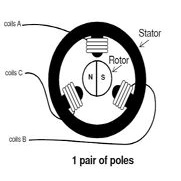
\includegraphics[width=\linewidth]{brushless-schematic}
            \end{center}
        \end{column}
    \end{columns}

\end{frame}

\imageframe[caption=Typical brushless motor,scale=0.9]{image81}


{\fullbackground[scale=0.9,page=5]{ian-brushless-dc-motors.pdf}
\begin{frame}{How do brushless motors work?}

%\begin{itemize}
%\item Electronic commutation is used to switch current in the stator could
%  so that the rotor is forced to rotate
%\item There is often a control magnet is in line with the poles of the large
%  magnet in the motor to identify rotor angle so that the controller can
%  switch current into the appropriate coils
%\item As it turns Hall sensors are stimulated by the magnetic flux.
%\item The Hall sensors are used to tell the controller what the orientation
%  is of the magnet with respect to the three winding phases.
%\item Current in the stator coils is turned on and off in sequence creating
%  motion from pole to pole.
%\end{itemize}

\end{frame}
}

\videoframe[0.65]{figs/brushless-commutation.mp4}

%{\fullbackground[scale=0.9,page=21]{../part1/figs/ian-sensors.pdf}
%    \begin{frame}{Electronic commutation systems}
%    \note {
%In this third part of the presentation we would like to understand the electronic commutation.
%There are different systems. maxon uses the following three :
%
%- Block commutation with or without Hall sensors
%- Sinusoidal commutation.
%
%As you can see the different maxon controller families perform different commutation types.
%
%Common to all these systems is that they should apply the current in a way, that the generated torque is as high as possible. As we have learned this is achieved by a perpendicular orientation of the magnetic fields of permanent magnet and winding. We have seen as well that we need to know the orientation of the permanent magnet to achieve this.
%
%We start with block commutation with Hall sensor position feedback. That's the standard commutation type. Once we have understood this the two other commutation schemes are easily derived from it.
%    }
%    \end{frame}
%}

{\fullbackground[scale=0.9,page=22]{../part1/figs/ian-sensors.pdf}
    \begin{frame}{Block commutation}

\pnote{
First we have to look at the Hall sensor feedback signals. Again we do this
based on the simplest design, the slotless maxon EC motor with 1 pole pair.

In the back of the motor there are three Hall sensor mounted on the PCB at an
angle of 120°. The Hall sensor detect the magnetic poles of the control magnet
which is mounted on the shaft. The control magnet exhibits the same two
magnetic poles in the same orientation as the power magnet. (Basically the Hall
sensors could monitor the power magnet directly but the control magnet offers
two advantages: The magnetic transitions between north and south pole are more
precisely defined. And an angular misalignment and tolerances between the
relative position of winding and Hall sensors can be adjusted.)

The digital Hall sensors used probe the direction of the magnetic field. They
generates a high output signal (5V) if the north pole of the control magnet is
close to them. A south pole produces a low level (Gnd).

The actual position of the control magnet in the diagram generates the
following signals:

- The blue Hall sensor sees the north pole. Thus the signal output level is
high and will remain high for the next 120°.
- The green Hall sensor is close to the south pole. The output level is low for
the next 60°. Then the north pole approaches and the output signal will switch
to a high state.
- The red Hall sensor has just switched from high to low where the signal level
will stay for the next half a turn.

The combination of the three Hall sensor signals is unique for each 60° of
rotation. Looking at these signals allows to know the rotor position within
60°. That exactly what we need for commutation. Remember there were 6 different
ways of current flow through the motor at a commutation angle of 60°.

The next slide shows how the complete block commutation system works.
}
    \end{frame}
}

{\fullbackground[scale=0.9,page=23]{../part1/figs/ian-sensors.pdf}
    \begin{frame}{Components of an EC drive system}
\pnote{
Let's first look at an EC drive system in general.

The three phases of the EC motor cannot be connected directly to a DC power
supply. The voltage needs to be switched in a sequence. This is done by the
electronic commutation. For the correct switching the electronics needs rotor
position information from the motor. This information is usually provided by
the Hall sensors.

An EC motor cannot operate on its own: It's always the combination of motor and
electronics commutation that makes the full drive.


For more sophisticated commutation and precise motor control, e.g. at very low
speeds, the use of an encoder feedback might be necessary. Often the
electronics not only performs the commutation but at the same time can be used
to control speed or position.
}
    \end{frame}
}



{\fullbackground[scale=0.9,page=7]{ian-brushless-dc-motors.pdf}
\begin{frame}{Brushless motor for RC aircraft}

\end{frame}
}

{\fullbackground[scale=0.9,page=8]{ian-brushless-dc-motors.pdf}
\begin{frame}{Construction of a EC brushless motor}

%Permanent magnet
%
%Special Winding
%
%Rotating part -- permanent magnet
%
%Hall sensors
%
%Control Magnet
%
%Case / Magnetic
%
%return

\end{frame}

}

{\fullbackground[scale=0.9,page=9]{ian-brushless-dc-motors.pdf}
\begin{frame}{Maxon EC flat brushless motor}

%Multi pole motor
%
%Flat design gives more torque as the flux is acting further from the
%centre of rotation

\end{frame}

}

{\fullbackground[scale=0.9,page=10]{ian-brushless-dc-motors.pdf}
\begin{frame}{Advantages and disadvantages of EC}

%\textbf{Brushed DC motors}
%
%\begin{itemize}
%
%\item Mechanical commutation
%\item Need periodic brush maintenance
%\item Power losses in brushes
%\item Sparking
%\item Can have noisy operation
%\item Linear torque characteristic at lower
%\item Change direction by changing voltage polarity
%\item Controller not always needed
%\end{itemize}
%
%\textbf{EC motors}
%
%\begin{itemize}
%
%\item Electronic commutation
%\item Low or no maintenance
%\item Less power loss
%\item No sparking
%\item Quieter operation
%\item More linear torque characteristic
%\item Change direction by changing switching sequence
%\item Always needs drive controller circuitry
%\item Requires sensors
%\item Higher reliability \& efficiency
%\item Stator on outside -- better for heat dissipation
%\item Longer life
%\item More expensive
%\end{itemize}

\end{frame}
}

%\section{Some other motors}
%
%\begin{frame}{Wound field motors}
%
%\begin{itemize}
%
%\item What happens if we apply AC to a permanent magnet DC motor?
%\end{itemize}
%
%\end{frame}
%
%\begin{frame}{Motor with stator winding}
%
%\end{frame}
%
%\begin{frame}{Shunt motor}
%
%\begin{itemize}
%\item Like DC motor but with electromagnet to generate static field
%\item Armature and field windings are connected in parallel
%\item Separate current through stator and armature
%\item Low Starting Torque
%\item Good Speed Regulation
%\item Used for fixed speed applications, windscreen wipers, fans
%\end{itemize}
%
%\end{frame}
%
%\begin{frame}{Shunt motor}
%
%Consider motor behavior under load:
%
%\begin{itemize}
%
%\item On application of load speed will reduce
%\item But this reduced armature EMF
%\item Therefore armature current rises
%\item Therefore torque increases
%\item So speed increases too
%\item Therefore system can do some self regulation of speed
%\item Much like permanent magnet DC motor!
%\end{itemize}
%
%\end{frame}
%
%\begin{frame}{Series motor}
%
%\begin{itemize}
%
%\item Armature and field windings are connected in series
%\item Same current goes through both
%\item High Starting Torque
%\item As the speed builds up so does the back EMF, reducing the current,
%  which causes a reduction in torque
%\item Poor Speed Regulation
%\item Used for starting heavy, industrial, high torque loads such as cranes,
%  hoists, elevators, trolleys and conveyors
%\item Cannot operate safely in an unloaded condition
%\end{itemize}
%
%\end{frame}
%
%\begin{frame}{Universal Motors}
%
%\begin{itemize}
%
%\item Series motor
%\item Uses field coils and not permanent magnets
%\item AC and DC operation
%\item As current direction changes it changes field direction on stator
%  field and also armature
%\item So always rotates in same direction independent of applied current
%  direction
%\end{itemize}
%
%\end{frame}



%%%%%%%%%%%%%%%%%%%%%%%%%%%%%%%%%%%%%%%%%%%%%%%%%%%%%%%%
%%%%%%%%%%%%%%%%%%%%%%%%%%%%%%%%%%%%%%%%%%%%%%%%%%%%%%%%
\miniframesoff
\begin{frame}{}
    \begin{center}
        \Large
        That's all, folks!\\[2em]

        \normalsize
        \textbf{Questions}:\\
        Portland Square B316 or \url{severin.lemaignan@plymouth.ac.uk} \\[1em]

        \textbf{Slides}:\\
        \href{https://github.com/severin-lemaignan/module-introduction-sensors-actuators}{\small
        github.com/severin-lemaignan/module-introduction-sensors-actuators} \\

        ...or the DLE!


    \end{center}
\end{frame}




\end{document}
